% A LaTeX template for EXECUTIVE SUMMARY of the MSc Thesis submissions to 
% Politecnico di Milano (PoliMi) - School of Industrial and Information Engineering
%
% P. F. Antonietti, S. Bonetti, A. Gruttadauria, G. Mescolini, A. Zingaro
% e-mail: template-tesi-ingind@polimi.it
%
% Last Revision: October 2021
%
% Copyright 2021 Politecnico di Milano, Italy. Inc. All rights reserved.

\documentclass[11pt,a4paper,twocolumn]{article}

%------------------------------------------------------------------------------
%	REQUIRED PACKAGES AND  CONFIGURATIONS
%------------------------------------------------------------------------------
% PACKAGES FOR TITLES
\usepackage{titlesec}
\usepackage{color}

% PACKAGES FOR LANGUAGE AND FONT
\usepackage[utf8]{inputenc}
\usepackage[english]{babel}
\usepackage[T1]{fontenc} % Font encoding

% PACKAGES FOR IMAGES
\usepackage{graphicx}
\graphicspath{{Images/}} % Path for images' folder
\usepackage{eso-pic} % For the background picture on the title page
\usepackage{subfig} % Numbered and caption subfigures using \subfloat
\usepackage{caption} % Coloured captions
\usepackage{transparent}

% STANDARD MATH PACKAGES
\usepackage{amsmath}
\usepackage{amsthm}
\usepackage{bm}
\usepackage[overload]{empheq}  % For braced-style systems of equations

% PACKAGES FOR TABLES
\usepackage{tabularx}
\usepackage{longtable} % tables that can span several pages
\usepackage{colortbl}

% PACKAGES FOR ALGORITHMS (PSEUDO-CODE)
\usepackage{algorithm}
\usepackage{algorithmic}

% PACKAGES FOR REFERENCES & BIBLIOGRAPHY
\usepackage[colorlinks=true,linkcolor=black,anchorcolor=black,citecolor=black,filecolor=black,menucolor=black,runcolor=black,urlcolor=black]{hyperref} % Adds clickable links at references
\usepackage{cleveref}
\usepackage[backend=biber,style=numeric]{biblatex}
\addbibresource{bibliography.bib}
% \usepackage[square, numbers, sort&compress]{natbib} % Square brackets, citing references with numbers, citations sorted by appearance in the text and compressed
% \bibliographystyle{plain} % You may use a different style adapted to your field

% PACKAGES FOR THE APPENDIX
\usepackage{appendix}

% PACKAGES FOR ITEMIZE & ENUMERATES 
\usepackage{enumitem}

% OTHER PACKAGES
\usepackage{amsthm,thmtools,xcolor} % Coloured "Theorem"
\usepackage{comment} % Comment part of code
\usepackage{fancyhdr} % Fancy headers and footers
\usepackage{lipsum} % Insert dummy text
\usepackage{tcolorbox} % Create coloured boxes (e.g. the one for the key-words)
\usepackage{stfloats} % Correct position of the tables

%-------------------------------------------------------------------------
%	NEW COMMANDS DEFINED
%-------------------------------------------------------------------------
% EXAMPLES OF NEW COMMANDS -> here you see how to define new commands
\newcommand{\bea}{\begin{eqnarray}} % Shortcut for equation arrays
\newcommand{\eea}{\end{eqnarray}}
\newcommand{\e}[1]{\times 10^{#1}}  % Powers of 10 notation
\newcommand{\mathbbm}[1]{\text{\usefont{U}{bbm}{m}{n}#1}} % From mathbbm.sty
\newcommand{\pdev}[2]{\frac{\partial#1}{\partial#2}}
% NB: you can also override some existing commands with the keyword \renewcommand

%----------------------------------------------------------------------------
%	ADD YOUR PACKAGES (be careful of package interaction)
%----------------------------------------------------------------------------
\usepackage{siunitx}
\usepackage[siunitx]{circuitikz}
\usepackage{stfloats}
\usepackage{tikz}
\usetikzlibrary{shapes.geometric, arrows, backgrounds, fit}
\ctikzset{bipoles/length=1.0cm}
\usepackage[autoload=true,
theme=grayscale-plain]{jlcode}

% To use with LuaLatex or XeTeX
% \usepackage{fontspec}

%----------------------------------------------------------------------------
%	ADD YOUR DEFINITIONS AND COMMANDS (be careful of existing commands)
%----------------------------------------------------------------------------
\lstdefinestyle{juliacode}{
  language=Julia, 
  showstringspaces=false,
  numbers=left,
  % stepnumber=1,
  numberstyle=\tiny,
  stepnumber=2,
  % numbersep=10pt,
  % Comment the following three lines to remove colors
  keywordstyle=\color{blue},
  commentstyle=\color{gray},
  identifierstyle=\color{purple!80},
  columns=fullflexible,
  keepspaces=true
}

\lstnewenvironment{juliacode}{\lstset{style=juliacode}}{}

%% To use with LuaLatex or XeTeX
% \newfontfamily \JuliaMono {JuliaMono-Light.ttf}[
%     Path      = ./,
%     Extension = .ttf
%     ]
% \newfontface \JuliaMonoLight{JuliaMono-Light}
% \setmonofont{JuliaMono-Light}[ Contextuals=Alternate ]

\tikzstyle{startstop} = [rectangle, rounded corners, minimum width=3cm, text width=3cm, minimum height=1cm,text centered, draw=black, fill=red!30]
\tikzstyle{process}   = [rectangle, minimum width=2cm, text width=3cm, minimum height=1cm, text centered, draw=black, fill=orange!30]
% \tikzstyle{process}   = [rectangle, draw=black, text width=3cm, fill=orange!30]
\tikzstyle{decision}  = [diamond, minimum width=2cm, minimum height=1cm, text centered, draw=black, fill=green!30]
\tikzstyle{image}     = [minimum width=1cm, minimum height=1cm, text centered]
\tikzstyle{arrow}     = [thick,->,>=stealth]


% Do not change ConfigExecutive/config.tex file unless you really know what you are doing. 
% This file ends the configuration procedures (e.g. customizing commands, definition of new commands)
\input{ConfigExecutive/config}

% Insert here the info that will be displayed into your Title page 
% -> title of your work
\renewcommand{\title}{Simulating Aeration at Birth: building an Open-Source Newborn Lung Model}
% -> author name and surname
\renewcommand{\author}{Luca Andriotto}
% -> MSc course
\newcommand{\course}{Biomedical Engineering - Ingegneria Biomedica}
% -> advisor name and surname
\newcommand{\advisor}{Prof. Prof. Raffaele Dellaca'}
% IF AND ONLY IF you need to modify the co-supervisors you also have to modify the file ConfigExecutive/title_page.tex (ONLY where it is marked)
\newcommand{\firstcoadvisor}{Dr. Chiara Veneroni} % insert if any otherwise comment
%\newcommand{\secondcoadvisor}{Name Surname} % insert if any otherwise comment
% -> academic year
\newcommand{\YEAR}{2023-2024}

%%% Local Variables:
%%% mode: LaTeX
%%% TeX-master: "../Executive"
%%% End:


\begin{document}

%-----------------------------------------------------------------------------
% TITLE PAGE
%-----------------------------------------------------------------------------
\input{ConfigThesis/title_page}

%-----------------------------------------------------------------------------
% TOC
%-----------------------------------------------------------------------------

% 1. Introduction
% 2. Capitolo sul Polmone dei Neonati (non visibile)
% 3. Anatomical Models
% 4. Mechanical Model of Airways and Acini
% 5. Model Development
%   5.1. Anatomical Model
%     5.1.1. CT Image Processing: Lung Segmentation, Centreline and Radii Extraction
%     5.1.2. Algorithmic Generation of the Distal Airway Centreline
%   5.2. Mechanical Simulator Model
%     5.2.1. Programming Language --- Model Designing & Instantiating
%     5.2.1.1  Callbacks' Role in State Variables Discontinuity Handling
%     5.2.3. Model Testing
% 6. Results
%   6.1. Anatomical
%   6.2. Mechanical Simulation
% 7. Conclusion and Future Development

% -----------------------------------------------------------------------------
% CHAPTERS
%-----------------------------------------------------------------------------
\section{Introduction}
\label{sec:introduction}
WIP.

% Commenti
% - Fragilità polmone neonatale
% - Differenze anatomiche tra neonato e adulto.
% - Albero bronchiale definizione etc. (penso anche ordini, branching etc).
% - Modello morfometrico definizione etc (?)
% - Modello polmone di agnello con capacità in parallelo.
% - Diametro trachea in funzione dell'eta gestazionale (grafico).

% \subsection{Premature newborns}
% \label{subsec:premature_newborns}

% Commenti
% Differenze tra sistema respiratorio nell'adulto e nel neonato e nel
% neonato prematuro.  (Slide 4 di [1]).

% \subsection{Morphometric Model}
% \label{subsec:morphometric_model}
% I am referring to \Cref{subsec:premature_newborns}

% \subsubsection{A brief definition}
% \label{subsubsec:morphometric_model_definition}

% Commenti
% Un'idea per questa definizione la si ritrova in
% `ModelloMorfometricoTriennale`.

% Commenti
% A morphometric model can be thought as a mathematical model composed
% by fixed parameters having both a physical and a geometrical (?)
% meaning.

% \subsubsection{Its structure}

% Slide 3 di [1]

% Riferimenti: `ModelloMorfometricoTriennale`,
% `ModelloMorfometricoTriennaleTesi`,
% `ModelloMorfometricoTriennaleBib/`

%%% Local Variables:
%%% mode: LaTeX
%%% TeX-master: "../Thesis"
%%% End:

% % 2. Capitolo sul Polmone dei Neonati (non visibile)
\section{Capitolo sul polmone dei neonati (lascia perdere per ora)}


%%% Local Variables:
%%% mode: LaTeX
%%% TeX-master: "../Thesis"
%%% End:

% 3. Anatomical Models
\section{Anatomical Models}
% - quello di agnello (al-jumaily2011)
% - un altro (herrmann2016)

% I modelli matematici sviluppati per i polmoni degli adulti non possono
% essere semplicemente ridotti in scala per adattarsi ai polmoni dei
% neonati. Infatti, i polmoni dei neonati non sono semplicemente una
% versione in miniatura dei polmoni degli adulti, ma presentano
% differenze significative in termini di proporzioni dei rami
% bronchiali, costituenti delle vie aeree, caratteristiche morfometriche
% e composizione. Queste differenze devono essere prese in
% considerazione quando si sviluppano o si adattano modelli matematici
% per rappresentare accuratamente il funzionamento dei polmoni dei
% neonati. La struttura dei polmoni dei neonati presenta proporzioni
% diverse rispetto a quella degli adulti. Le diramazioni delle vie aeree
% possono avere dimensioni e disposizioni differenti.  I componenti dei
% polmoni, come il tessuto e le cellule, possono variare tra neonati e
% adulti.  Gli studi morfometrici, che analizzano la forma e la
% struttura dei polmoni, mostrano che ci sono differenze tra neonati e
% adulti che devono essere considerate nei modelli.  Ci sono differenze
% nella composizione del tessuto polmonare tra neonati e adulti che
% influenzano come i polmoni funzionano e rispondono alle terapie.

% The hierarchy of the dividing airways largely determines the internal
% lung structure, which is a fractal branching tree\cite{suki2011}. The
% structural design of the airway tree is functionally important because
% the branching pattern plays a role in determining air flow and
% particle deposition. In modeling the human airway tree, it is
% generally agreed that the airways branch according to the rules of
% irregular dichotomy.  Regular dichotomy means that each branch of a
% treelike structure gives rise to two daughter branches of identical
% dimensions. In irregular dichotomy, however, the daughter branches may
% differ greatly in length and diameter.

The structure of the internal lung is significantly influenced by the
hierarchical arrangement of the airways, which resemble a fractal
branching tree\cite{suki2011}. The design of this airway tree is
crucial for its function, as the branching pattern affects both
airflow and particle deposition. In modeling the human airway tree, it
is widely accepted that the airways follow an irregular dichotomy
pattern. Unlike regular dichotomy, where each branch splits into two
identical daughter branches, irregular dichotomy results in daughter
branches that can vary significantly in length and diameter.

\begin{figure}[H]\centering
  % \includegraphics[width=\textwidth]{airway_tree_best.jpg}
  \includegraphics[width=.8\textwidth]{airway_tree_no_left_best.jpg}
  \caption{Representation of the major airways.}
  \label{fig:airway_tree_anatomical}
\end{figure}

Mathematical models developed for adult lungs cannot simply be scaled
down to fit the lungs of newborns. In fact, newborn lungs are not
simply one miniature version of adult lungs, but they present
significant differences in terms of bronchial branch proportions,
constituents of the airways\cite{merkus1996}, morphometric
characteristics\cite{horsfield1987} and
composition\cite{hislop1989}. These differences must be taken into
account when developing or adapting mathematical models to accurately
represent the functioning of the lungs of the newborns. The structure
of the lungs of newborns presents proportions different than that of
adults. The branches of the airways they can have different sizes and
arrangements. The components of lungs, like tissue and cells, can vary
between newborns and adults. Morphometric studies, which analyze the
shape and the structure of the lungs, show that there are differences
between newborns and adults that need to be considered in the
models\cite[][Ch. 1.1]{mani2020}. There are differences in the
composition of lung tissue between newborns and adults who influence
how the lungs function and respond to therapies.

%% Citare qui i riferimenti che ha fatto chiara nella call del 21.06

\textcite{mani2020} considered an adult lung model linearly scaled to
match newborn anatomical features.  The advantage of this approach is
that it respects the dimensions of trachea and bronchioles. It doesn't
guarantee that the morphometric characteristics of the entire airway
tree are respected.  In this work, there are few airway generation
parameters that can in fact be adapted, in order to better approximate
the target morphometric characteristics.

% Modello ovino (al-jumaily2011) e di Jacob (herrmann2016).

% GESTISCI IMMAGINE E TESTO SOTTO
\begin{figure}[H]\centering
  \includegraphics[width=.5\textwidth]{albero_dicotomico_best.png}
  \caption{The dichotomous bronchial tree.}
  \label{fig:albero_dicotomico_anatomical}
\end{figure}

% Prendo quest'immagine e spiego che l'albero che sto considerando può
% essere modellizzato come un albero dicotomico, cioè che si divide
% sempre in due ed in cui sono sempre diversi gli angoli, le lunghezze,
% possono avere diramazioni diverse e quindi proprietà diverse.

% AGGIUNTA QUESTA MODIFICA, COMPLETARE
% -> spiegato il concetto in inglese.
\Cref{fig:albero_dicotomico_anatomical} serves as a reference for
constructing anatomically coherent adult lungs. In a dichotomous tree,
each airway (excluding the trachea) has a single parent branch and two
daughter branches (excluding the acini).  Asymmetrical bronchial trees
are a specific class presenting uneven splitting: Horsfield orders of
two siblings are in fact different (causing recursion index $\Delta$
to exist, see \cref{fig:airway_impedance}).  Branching angles, lengths
and diameters can vary, resulting then in different mechanical
properties.

Newborn lung can be considered as having an analogous structure.

% LEGGERE INTRONORA E TAWHAI, POI CAPIRE COME CITARLI IN QUESTO PUNTO.
Da tac, .. estratto centerline e ricostruito con diversi algoritmi la parte
mancante (Nora, Tawn..).

% Questa struttura in \Cref{fig:albero_dicotomico_anatomical} è stata
% usata come riferimento per la costruzione di alberi brochiali
% anatomicamanete coerenti per applicazioni su adulti. 

% PER CITARE NORA: \cite{tgavalekos2003}, PER CITARE TAWHAI
% \cite{tawhai2000}

Instead for infants, there exist models based on the
ovine\cite{al-jumaily2011} and canine\cite{herrmann2016} anatomy.

%%% Local Variables:
%%% mode: LaTeX
%%% TeX-master: "../Thesis"
%%% End:

% 4. Mechanical Model of Airways and Acini
\section{Mechanical Model of Airways and Acini}

% (cambiare `acini`) (paper in chat Lutchen). (no zsoft e
% cartilagine)

% Scrivere in breve la struttura circuitale che poi implemento
% (copia).

% La struttura circuitale è descritta in lutchen1997 in marrone.

The adult airway can be likened to a transmission line (see
\cref{fig:airway_impedance}), with resistors, capacitors and inductors
having constant values.  These components form a circuit as
illustrated.  Moreover, tissues properties ($Z_{\text{w}}$) are
incorporated.  \Cref{fig:airway_impedance,fig:acinus_impedance} are
modules connected according to the structure of newborn airway, which
is comparable to that depicted in
\Cref{fig:albero_dicotomico_anatomical}.  $Z(n)$ represents the parent
branch as a function of the Horsfield order, while $Z(n-1)$ and
$Z(n-1-\Delta)$ denote the two daughters branches.  $Z(2)$ represents
the terminal airway.  Each airway has a parent branch (excluding the
trachea) and two daughter branches (excluding the acini).

% L'equivalente elettrico delle proprietà dei tessuti è stato modificato
% per poter testare l'impatto delle modifiche fisiologiche durante il
% processo di aereazione.

The electrical equivalent of tissues properties is modified to test
the physiological change impact on aeration process.

% Inoltre, il liquido fetale è incomprimibile, l'aria invece non lo è,
% comportando la presenza di un elemento aggiuntivo nell'equivalente
% elettrico dell'aria, in quanto la compressibilità del gas è
% modellizzata attraverso una capacità. In aggiunta, bisogna tener conto
% del collasso delle vie aeree, perché durante il processo di aerazione
% si crea un'interfaccia aria-liquido, che a sua volta dà origine a una
% tensione superficiale, la quale deve essere superata per permettere lo
% spostamento del fluido nell'albero bronchiale.  Una volta superata, i
% diametri si possono ingrandire facendo aumentare il volume polmonare.

Air-fluid interface modulates the values of resistances and
inductances in both the modules types.

Moreover, this fluid is incompressible, whereas air is not. This
introduces an additional element in the electrical equivalent of air,
as the compressibility of the gas is modeled through a
capacitance.

% Additionally, it is necessary to consider the collapse of
% the airways.

During the aeration process, an air-liquid interface is created, which
in turn generates surface tension that must be overcome to allow fluid
movement within the bronchial tree. Once this surface tension is
overcome, the diameters can expand, leading to an increase in lung
volume.

\textcite{lutchen1997} have developed a mechanical lung model in
frequency-domain, describing airways and acini modules as displayed
in \cref{fig:airway_impedance} and \cref{fig:acinus_impedance},
respectively.

% Circuiti copiato da lutchen1997. 
\begin{figure}[H]\centering
  \begin{circuitikz}[scale=1]
    % Circuit
    %% Main branch
    %%% Input Node
    \draw (1.5,0)
    node[ocirc] (circuit_IN) {}
    to[short, ] ++(1,0) coordinate(R_IN)
    ;
    
    %% Main branch
    \draw (R_IN)
    to[short] ++(.5,0)
    to[resistor, l=$R(n) / 2$] ++(1,0)
    to[inductor, l=$I(n) / 2$] ++(3,0) coordinate (C_g_IN)
    to[short] ++(1.5,0) coordinate (SW_IN)
    to[resistor, l=$R(n) / 2$] ++(3,0)
    to[inductor, l=$I(n) / 2$] ++(1,0)
    to[short, -*] ++(1,0) coordinate(circuit_OUT)
    ;

    %%% C_g branch
    \draw (C_g_IN)
    to[polar capacitor, invert, l_=$C_{\text{g}}(n)$, *-] ++(0,-3.5)
    node[ground]{} ++(0,0)
    ;

    %%% Zw branch
    \draw (SW_IN)
    to[twoport, t={$Z_{\text{w}}(n)$},bipoles/twoport/height=1.2, *-] ++(0, -3.5)
    node[ground]{} ++(0,0)
    ;

    \draw (circuit_OUT)
    -- ++(0, .5)
    to ++(1.88,0)
    node[draw, anchor=west, thick] {$Z(n-1)$};
    
    \draw (circuit_OUT)
    -- ++(0, -.5)
    to ++(1,0)
    node[draw, anchor=west, thick] {$Z(n-1-\Delta$)};

    % Nodes
    %% IN
    \draw[->, >=stealth, thick] (0,0) -- (circuit_IN) node[midway, above] {Z(n)};
  \end{circuitikz}
  \caption{Impedance ($Z$) of a given order ($n$) of a single airway
    generation is calculated via an acoustic transmission line
    analysis, which accounts for shunting into gas compression in the
    tube ($C_{\text{g}}(n)$) and into nonrigid airway walls
    ($Z_{\text{w}}$).  R: resistance; $\Delta$: recursion
    index\cite{lutchen1997}.}
  \label{fig:airway_impedance}

\end{figure}

%%% Local Variables:
%%% mode: LaTeX
%%% TeX-master: "../Thesis"
%%% End:

\begin{figure}[H]\centering
  \begin{circuitikz}[scale=.9]
    % Circuit
    %% Main branch
    %%% Input Node
    \draw (1.5,0)
    node[ocirc] (circuit_IN) {}
    to[short, ] ++(1,0) coordinate(Z_IN)
    to[twoport, bipoles/twoport/width=1.0, t=$Z(2)$] ++(2,0) coordinate(C_g_IN)
    ;
    
    %% Main branch
    % \draw (Z_IN)
    % to[twoport, t=$Z_{2}$] ++(2,0) coordinate(C_g_IN)
    % ;

    %%% C_g branch
    \draw (C_g_IN)
    to[polar capacitor, invert, l_=$C_{\text{g}}(n)$, *-] ++(0,-3.5)
    node[ground]{} ++(0,0)
    ;

    %%% Zw branch
    \draw (C_g_IN)
    to[inductor, l=$I_{\text{t,i}}$] ++(2, 0)
    to[twoport, t={$\dfrac{G - j\cdot H}{\omega^\alpha}$},bipoles/twoport/width=2.0, bipoles/twoport/height=1.2] ++(3, 0)
    to[short] ++(0, -3.5)
    node[ground]{} ++(0,0)
    ;

  \end{circuitikz}
  \caption{An alveolar-tissue element is attached to the terminal
    airways in the tree. There is gas compression corresponding to
    volume of the acinus ($C_{\text{g}}$) and the tissue element is
    viscoelastic containing a tissue damping ($G$) coupled to
    elastance ($H$) to ensure a constant tissue hysteresis. $j$:
    imaginary unit, $I_{\text{t,i}}$: tissue
    inertance\cite{lutchen1997}.}
  \label{fig:acinus_impedance}

\end{figure}

%%% Local Variables:
%%% mode: LaTeX
%%% TeX-master: "../Thesis"
%%% End:


In this thesis, as well as in \cite{mani2020}, a mechanical model is
defined in time-domain starting from the modules described in this
section and properly adapted.

% AGGIUNTA MODIFICA, COMPLETARE
% -> la parte sul fluido è stata inserita sopra
% -> la parte del diodo è stata inserita sotto.

% In questo punto devo inserire la spiegazione del modello in cui si
% inserisce anche il diodo, oltre al liquido. proprio perché mani2020
% è stata la prima ad inserirlo.

% liquido .. diodo

Capillary pressure is due to air-fluid interface in the airway tree.
It was taken into account and modeled as a diode component: opening
threshold voltage is correspondent to aforementioned capillary
pressure for a generic airway.

% Da spostare in implementation? 
A first implementation has been performed on «CADENCE» platform.  This
has the advantage of parallelism and speed.  There are also some
drawbacks to this approach: this framework is designed to simulate
standard electrical components and it is not well-suited to develop
time- and current integral-dependent components.  Furthermore license
is proprietary and machine specific.  This limits the accessibility of
of model design process.

% Posso dire che l'alveolo è stato modificato (vedi Veneroni2024) a
% partire dall'alveolo mostrato da lutchen1997 perché non risolvibile
% nel dominio del tempo.

%%% Local Variables:
%%% mode: LaTeX
%%% TeX-master: "../Thesis"
%%% End:

% 5. Model Development
%   5.1. Airway Tree
%     5.1.1. CT Image Processing: Lung Segmentation, Centerline and Radii Extraction
%     5.1.2. Generation of the Statistical Portion
%   5.2. Mechanical Simulator
%     5.2.1. Blocks Description
%     5.2.2. Callbacks' Role in State Variables Discontinuity Handling
%     5.2.3. Model Testing on A Subtree
\section{Model Development}
% Mettere enfasi sulla ricerca dei metodi perché Julia e non altro.

% Visione d'insieme (diagramma con flusso dell'informazione, data
% pipeline). Questo diagramma mostra a partire dagli input che ho
% avuto (TC) tutto l'iter del dato.

% Qui ha detto poi Chiara che conviene inserire delle informazioni
% riguardanti i modelli matematici utilizzati.

\Cref{fig:data_pipeline} provides a high-level overview of the main
operations performed.

% Each of the two classes of methods corresponds to one of the two
% models:

% \begin{enumerate}
% \item \emph{Chaste} library is utilized in the generation of
%   \emph{morphometric model}.
% \item \emph{Julia Programming Language} is employed to describe and
%   instantiate the \emph{mechanical model}, as well as to perform
%   \emph{simulations}.
% \end{enumerate}

% todo: modificare l'immagine sopra ad "anatomical surrogate generation" con uno screen di ParaView.
% todo: aggiungere immagini sopra al branch del modello meccanico.

\begin{figure}[H]\centering
  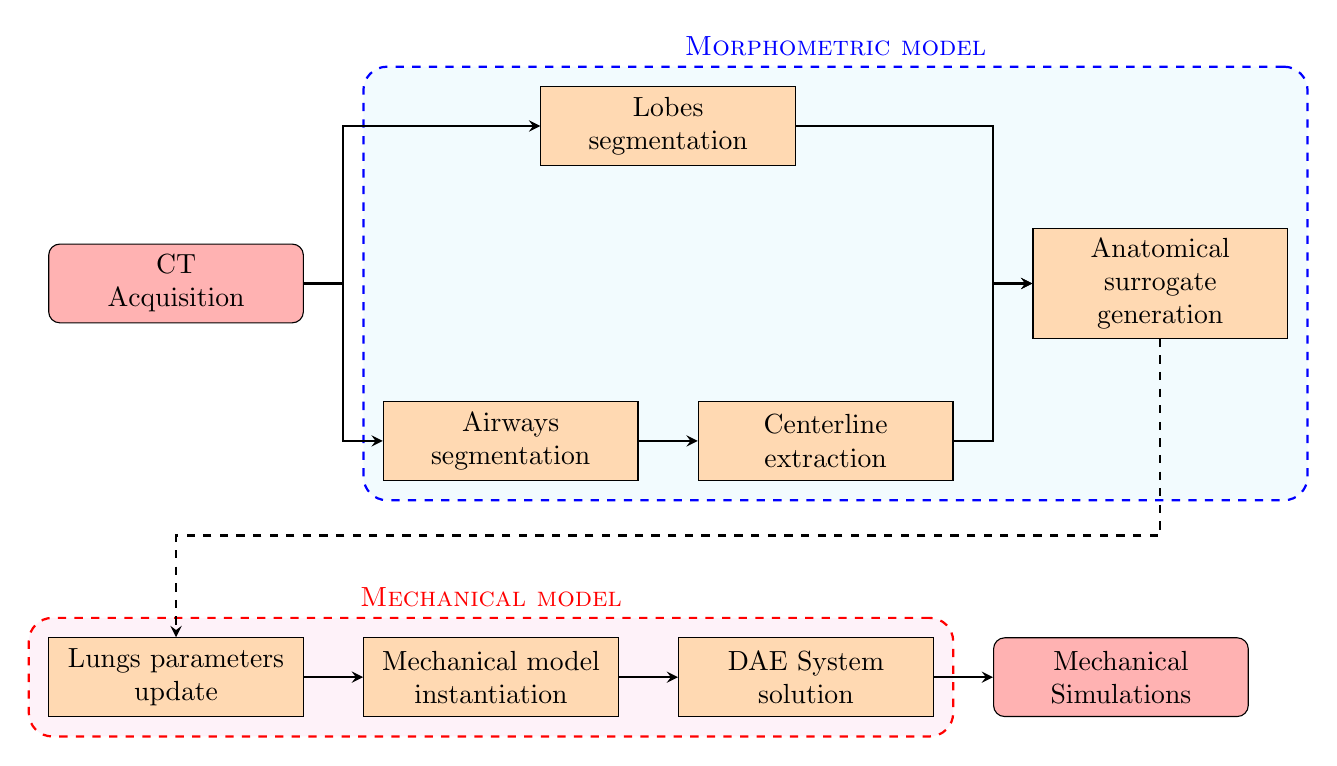
\begin{tikzpicture}[node distance=3cm]
    % Nodes
    %% Chaste & Morphometric Model
    \node (ct_acquisition)           [startstop] {CT\\Acquisition};
    % \node (img_ct_acquisition)       [image, above of=ct_acquisition, yshift=-1.0cm]                   {\includegraphics[width=2.0cm]{ct_acquisition.png}};
    %%% Upper branch
    \node (lobes_segmentation)       [process, right of=ct_acquisition, xshift=3.25cm, yshift=+2cm]    {Lobes\\segmentation};
    %%% Lower branch
    % \node (img_lobes_segmentation)   [image, above of=lobes_segmentation, xshift=-.1cm, yshift=-1.2cm] {\includegraphics[width=3.5cm]{lobes_segmentation.png}};
    \node (airways_segmentation)     [process, below of=lobes_segmentation, xshift=-2cm, yshift=-1cm]  {Airways\\segmentation};
    % \node (img_airways_segmentation) [image, above of=airways_segmentation, xshift=2cm, yshift=-1cm]   {\includegraphics[height=2.5cm]{airways_segmentation.png}};
    \node (centerline_extraction)    [process, below of=lobes_segmentation, xshift=+2cm, yshift=-1cm]  {Centerline\\extraction};
    \node (surrogate_generation)     [process, right of=ct_acquisition, xshift=9.5cm]                  {Anatomical surrogate\\generation};
    % \node (img_surrogate_generation) [image, above of=surrogate_generation, yshift=-.5cm]              {\includegraphics[width=3.5cm]{lobes_segmentation.jpg}};
    %% Julia & Mechanical Model
    \node (parameters_update)        [process, below of=ct_acquisition, yshift=-2cm]                   {Lungs parameters\\update};
    \node (model_instantiation)      [process, right of=parameters_update, xshift=1cm]                 {Mechanical model\\instantiation};
    \node (DAE_solution)             [process, right of=model_instantiation, xshift=1cm]               {DAE System\\solution};
    \node (simulations)              [startstop, right of=DAE_solution, xshift=+1cm]                   {Mechanical Simulations};

    % Arrows
    \draw [arrow] (ct_acquisition.east)                              -- ++(.5,0) coordinate(tmp)     |- (airways_segmentation.west);
    \draw [arrow] (airways_segmentation)                             -- (centerline_extraction);
    \draw [arrow] (centerline_extraction.east)                       -- ++(.5,0) coordinate(tmp1)    |- (surrogate_generation.west);
    \draw [arrow] (model_instantiation)                              -- (DAE_solution);
    \draw [arrow] (DAE_solution)                                     -- (simulations);
    \draw [arrow] (tmp)                                              |-   (lobes_segmentation.west);
    \draw [arrow] (lobes_segmentation)                               --   (tmp1|-lobes_segmentation) |- (surrogate_generation.west);
    \draw [dashed, thick, ->,>=stealth] (surrogate_generation.south) -- ++(0,-2.5)                   -| (parameters_update.north);
    \draw [arrow] (parameters_update)                                -- (model_instantiation);

    % Frame around a part of the flowchart
    \begin{pgfonlayer}{background}
      \node[rounded corners=3mm,
      draw=blue,
      thick, dashed,
      % fit=(airways_segmentation)(centerline_extraction)(img_lobes_segmentation)(img_surrogate_generation),
      fit=(airways_segmentation)(centerline_extraction)(lobes_segmentation)(surrogate_generation),
      fill=cyan!5,
      inner sep=7pt,
      label={[anchor=south]above:\textsc{\textcolor{blue}{Morphometric model}}}] {};
    \end{pgfonlayer}
    \begin{pgfonlayer}{background}
      \node[rounded corners=3mm,
      draw=red,
      thick, dashed,
      fit=(parameters_update)(model_instantiation)(DAE_solution),
      fill=magenta!5,
      inner sep=7pt,
      label={[anchor=south]above:\textsc{\textcolor{red}{Mechanical model}}}] {};
    \end{pgfonlayer}
  \end{tikzpicture}
  \caption{Data pipeline.  The process begins with a
    \emph{patient-specific image} (i.e. CT) of a premature newborn.
    The extracted data, comprising \emph{two segmentations}, are then
    processed to obtain an anatomical surrogate of the airway tree.
    This is necessary due to scanner resolution not allowing for the
    discrimination and localization of small branches.  From the
    resulting morphometric model, the \emph{mechanical parameters} can
    be derived, which are essential for generating an accurate
    simulation model.  Finally, a numerical solver for differential
    equations provides the final output.}
    \label{fig:data_pipeline}
\end{figure}

%%% Local Variables:
%%% mode: LaTeX
%%% TeX-master: "../Thesis"
%%% End:


%   2.2. Morphometric model
\subsection{Airway Tree}
\label{subsec:airway_development}
% Per Chiara: Inserisco definizione di modello morfometrico?
There are different open-source platforms available for generating morphometric models.  In particular:

\begin{enumerate}
\item AVATree (Windows-only)
\item Chaste (crossplatform) library
\end{enumerate}

Due to problems related to «AVATree» source code compilation for
Windows with «VisualStudio», Chaste library is selected for this
project.

Chaste is a C++ open-source (BSD licensed) library developed by Oxford
University.  It has multiple use cases across various biomedical
fields, with an emphasis on cardiac electrophysiology and cancer
development\cite{mirams2013}.  It can be integrated into a C++ program
or used via «User Project» (i.e. \texttt{ctest}).  Specifically, the
``AirwayGenerationTutorial'' is considered as a first codebase and
properly adapted to match newborn
parameters\cite{airwaygeneration2024}.

The required input consists of two pieces of information:
\begin{itemize}
\item A \emph{mesh of centerline points}.  This mesh is provided in
  TetGen format, comprising ``airways.node'' and ``airways.edge''
  files. The first file lists centerline points coordinates,
  respective sampled airways radius and a boolean value to indicate if
  the point is generative. The second one contains all the connections
  between pairs of points.
\item Four (or five) \emph{lobes segmentations} in STL format.  These
  segmentations are necessary as they physically impose a limit on the
  growth algorithm.
\end{itemize}

%     2.2.1. CT, centerline and radii extraction
\subsubsection{CT Image Processing: Lung Segmentation, Centerline and
  Radii Extraction}
\label{subsubsec:ct_centerline_radii_extraction}
% todo: Devo chiedere bene a Francesca come sono stati estratti i
% raggi.

«3D Slicer» is an open-source software used for CT image processing.
Two extensions are installed:

\begin{description}
\item «\emph{Chest\_imaging\_platform}»: This extension enables
  semi-automatic segmentation of major airways from a single fiducial
  point.  It can also extract adult lobes using three fiducial points
  per lung fissure. However, in our case, the fissures are not
  visible, necessitating manual intervention.
\item «\emph{SlicerVMTK}»: This extension is used for extracting
  centerline points.
\end{description}

%     2.2.2. Generation of the statistical part
\subsubsection{Generation of the Statistical Portion}
\label{subsubsec:statistical_generation}

The Chaste User Project reads the input files
(see \Cref{subsec:airway_development}), and begins growing the
anatomical surrogate from the points labeled as «generative».  The
algorithm operating under the hood is a modified version of the one
described in \cite{tawhai2000,bordas2015}.  The generated output is
available in various formats:

\begin{itemize}
\item vtu: Unstructured Grid (base64 encoded) format used by VTK
  library.  It can be displayed by ParaView, an open-source viewer.
\item node and edge: TetGen format.  Such files are better suited for
  further processing.
\end{itemize}

% bordas2015 parla anche di come vengono generate le vie aeree e come
% vengono assegnati i diametri.

% Riferirsi a tawhai2000 e bordas2015.
This process is required as it is not possible to obtain high
generations (aka small airways) by means of standard high-resolution
CT\cite{bordas2015}.

The algorithm is based on a modified version of \textcite{tawhai2000}.
% {1} va spiegato qui, poi descriviamo l'algoritmo
A uniform grid of seed points is created within each segmented lobar
surface. Seed points approximately correspond to terminal bronchioles.
Spacing of the seed point grid is set so that the mean volume around
each of such points corresponded to the acinar volume (for adult being
$187\text{mm}$).

The starting points of the algorithm are the distal ends of the
segmented airway centerlines.  These points are referred to as growth
apices.

An \emph{adaptive threshold} on the distance between the seed points
and growth apices is required to prevent spurious long airways being
generated in the last few generations.  \Cref{eq:airway_threshold}
describes such threshold:

\begin{equation}
  T = \max(V_{\text{b}} - n\cdot D_{\text{l}}, 5\text{mm})
  \label{eq:airway_threshold}
\end{equation}

Where:
\begin{description}
\item $V_{\text{b}}$ is the diagonal size of the bounding box of the lobe being
  generated into
\item $D_{\text{l}} (= {V_{\text{b}}/{N}})$ is the distance limit.
\item $N$ is the maximum number of generations.
\item $n$ is the current generation number.
\end{description}

With these definitions, the \textbf{growing algorithm} is described as
such:

\begin{enumerate}
\item \emph{Each seed point is associated to the closest growth apex
    within its lobe}.  Seed point having a distance with respect to a
  growth apex greater than the aforementioned adaptive threshold is
  not associated to that distal end.  If all distal ends are further
  than the threshold from the seed point, the seed point remains
  unlabeled.
\item \emph{Calculation of the centroid of points assigned to each
    distal branch.}
\item \emph{The plane defined by the centroid and the parent branch is
    used to split the points into two unequal sets.}
\item \emph{Centroids of each of the new point sets are calculated.}
\item \emph{For each set of points a new airway is generated} starting
  at the distal end and extending 40\% of the distance towards the
  centroid of the point set.
\item \emph{Generated branches are checked to determine whether it is
    terminal}.  Branches whose length is less than $2\text{mm}$ are
  considered terminal.  Also branches whose point set contains just a
  single point solely are considered terminal points.  For all
  terminal branches their associated seed point is discarded from the
  global set.
\item \emph{Iterate} until no seed point is available.
\end{enumerate}

\textbf{Diameters} are computed by means of \Cref{eq:lumen_diameter}.

\begin{equation}
  \log D(x) = (x - N)\log(R_{\text{d}} H) + \log(D_{\text{N}})
  \label{eq:lumen_diameter}
\end{equation}

Where:
\begin{description}
\item $D$ is the aiway diameter.
\item $x$ is the current Horsfield order.
\item $N$ is the maximum Horsfield order.
\item $D_{\text{N}}$ is the maximum diameter.
\item $R_{\text{d}} H$ is the anti-log of the slope of airway diameter
  plotted against Horsfield order and is set to 1.15.  This parameter
  in the code is named ``DiameterRatio''.
\end{description}
  
%   2.3. Julia Programming Language
\subsection{Mechanical Simulator}
\label{subsec:simulator_development}

In order to perform simulation it is required to use an efficient
differential equation solver.  «DifferentialEquations.jl» wraps all
available solvers (even C and Fortran ones) and it is very efficient
\cite{diffeqdocs2024,rackauckas2017}.

Julia is a free, open-source (MIT licensed), fast, scientific and
numerical computing-oriented programming language.  Its computational
efficiency is comparable to that of statically-typed languages like C
or Fortran.  Moreover, its high-level code expressivity rivals that of
languages like Python, R and MATLAB\cite{juliadocs2024}.

Two key features, inspired by the \emph{Lisp Language}, are
highlighted here.

\begin{description}
\item \emph{Metaprogramming}: Code is treated as any other Julia data
  structure, thus can be dynamically generated and manipulated at
  runtime.
\item \emph{Macros}: They help instantiate the generated code in the
  body of a program.
\end{description}

Their importance is closely tied to the concept of Domain-Specific
Languages (aka DSLs).  These dialects are composed by abstractions
that can be properly exploited to solve particular problems
(e.g. modeling complex systems, solving differential equations).

Julia REPL has a built-in package manager (i.e. «\texttt{Pkg.jl}»)
used for managing project dependencies and ensuring the
\emph{repeatability} of computational setups.  This is achieved by
saving the required package names and commits into `Project.toml' and
`Manifest.toml' files.

%     2.3.1. «ModelingToolkit.jl» handles model complexity
\subsubsection{«\texttt{ModelingToolkit.jl}» handles
  Model Complexity}
\label{subsubsec:modelingtoolkit}

This Julia package encompasses all the tools necessary for model
design.  \texttt{ModelingToolkit.jl}» is equation-driven, requiring
each system to be described by Differential-Algebraic Equations
(i.e. DAEs) for subsequent solving\cite{ma2021}. Its built-in DSL
optimizes every stage of modeling, from prototyping components to
instantiating the complete system.

An acausal paradigm can be adopted, allowing users to reason in terms
of \emph{components}\cite{mtkdocs2024}. This modularity facilitates
system extensibility compared to the causal approach, where the entire
system of Differential-Algebraic Equations must be considered and
manually simplified\cite{ma2024}.

In particular, the usage of \jlinl{@mtkmodel} macro enables
hierarchical generation of building blocks recurring in the
highest-order model (i.e. «Lungs»).  Here is how information is
structured within \jlinl{@mtkmodel} macro.

\begin{jllisting}[label=@mtkmodel, caption={\jlinl{@mtkmodel}: a macro for systems prototyping.}]
  @mtkmodel <name_of_model> begin
      @parameters begin
          # (Optional) Some constant (e.g. Resistance, Capacitance) ...
      end
      @components begin
          # (Optional) Some dependency system (e.g. Resistor, Capacitor) ...
      end
      @variables begin
          # (Optional) Internal variables ...
      end
      @equations begin
          # Differential Algebraic Equations describing the model's behavior.
      end
      @continuous_events begin
          # (Optional) Some callback function ...
      end
  end
\end{jllisting}

Replicating the behavior of electrical components using this language
is straightforward, once you are familiar with the syntax and
understand the Differential-Algebraic Equations that represent their
characteristics.  Each generated system can then be composed into more
complex ones, using the internal \jlinl{@components} macro, thereby
implementing the hierarchical structure mentioned earlier.

After describing the highest-order system, Julia compiler requires its
instantiation before any simulation can be performed.  This is
accomplished using \jlinl{@mtkbuild} macro, which minimizes the number
of equations that need to be solved.

%     2.4.1. Blocks description
\subsubsection{Blocks Description}
\label{subsubsec:blocks_description}

Code modularity is directly reflected in the electrical equivalent
circuit.  Specifically, by encapsulating systems with the internal
\jlinl{@components} macro, it becomes possible to generate models of
increasing complexity.  This approach enables a clear separation
between components belonging to different hierarchical levels and
facilitate compartmentalization during the model design phase.

% 1. È necessario indicare la notazione utilizzata nelle formule?
% 2. Su cosa devo concentrarmi nella descrizione? Devo mostrare
% codice?

The following blocks are listed in a bottom-up order (from lowest to
highest).

\begin{enumerate}
\item \textbf{Electrical components}.  The simplest blocks are derived
  from «\texttt{ModelingToolkitStandardLibrary}», while
  integral-dependent ones rely on a modified mathematical block to
  manage both current integration and its timing correctly.  Their
  behavior varies based on the neonatal pulmonary fluid interface.
  \begin{itemize}
  \item \emph{Current Integral-Dependent Inductor}:
    $L(t) = L_{a} + L_{b}\cdot \left(1 - \dfrac{\int {i
          dt}}{V_{\text{FRC}}}\right)$
  \item \emph{Current Integral-Dependent Resistor}:
    $R(t) = R_{a} + R_{b}\cdot \left(1 - \dfrac{\int {i
          dt}}{V_{\text{FRC}}}\right)$
  \item \emph{Diode}
  \item \emph{Inductor}
  \item \emph{Resistor}
  \end{itemize}
\item \textbf{Modules}.  Obtained by connecting the aforementioned
  components together into functional models representing a
  physiological structure.
  \begin{itemize}
  \item
    \emph{Alveolus}
  \item \emph{Airway}.  It has a similar behavior with respect to a
    transmission line.
  \end{itemize}
\item \textbf{Lungs}.  Highest order model as it is a combination of
  alveoli and airways.
\end{enumerate}

% Equivalent circuits for airways and alveolus.
\begin{figure}[H]\centering
  \begin{circuitikz}[]
    % Circuit
    %% Main branch

    %%% Input Node
    \draw (1.5,0)
    node[ocirc] (circuit_IN) {}
    to[short, i=$i_{\text{in}}$, -*] ++(1.5,0) coordinate(D_SW_IN)
    ;
    
    %%% Diode // Switch branch
    \draw (D_SW_IN)
    to[short] ++(0,.5)
    to[diode, v^<=$V_{\text{in,th}}$, color=bluePoli] ++(2,0) coordinate(D_SW_OUT)
    to[short, -*] (D_SW_IN-|D_SW_OUT)
    ;
    \draw (D_SW_IN)
    to[short] ++(0,-.5)
    to[switch, color=bluePoli, a_=$\left(V_{\text{in}}\geq V_{\text{in,th}}\right) \lor \left(V_{\text{in}} \text{ = } 0\right)$] ++(2,0)
    to[short] (D_SW_IN-|D_SW_OUT)
    ;

    %% Main branch
    \draw (D_SW_IN-|D_SW_OUT)
    to[short] ++(.5,0)
    to[variable resistor, color=bluePoli, l=$R_{\text{tube}} / 2$] ++(2,0)
    to[variable inductor, color=bluePoli, l=$I_{\text{tube}} / 2$] ++(2,0) coordinate (C_g_IN)
    to[short] ++(1.5,0) coordinate (SW_IN)
    to[variable resistor, color=bluePoli, l=$R_{\text{tube}} / 2$] ++(2,0)
    to[variable inductor, color=bluePoli, l=$I_{\text{tube}} / 2$] ++(2,0)
    to[short, i=$i_{\text{out}}$] ++(1,0)
    node[ocirc] (circuit_OUT) {}
    ;

    %%% C_g branch
    \draw (C_g_IN)
    to[C=$C_{\text{g}}$, *-] ++(0,-3.5)
    node[ground]{} ++(0,0)
    ;

    %%% Sw branch
    \draw (SW_IN)
    to[L=$I_{\text{sw}}$, *-] ++(0,-1.5)
    to[R=$R_{\text{sw}}$] ++(0,-1)
    to[C=$C_{\text{sw}}$] ++(0,-1)
    node[ground]{} ++(0,0)
    ;
    
    %% Open circuit (input)
    \draw (circuit_IN)
    to[open, -o, v<=$V_{\text{in}}$] ++(0, -3.5)
    node[ground] {}
    ;
    %% Open circuit (output)
    \draw (circuit_OUT)
    to[open, -o, v^<=$V_{\text{out}}$] ++(0, -3.5)
    node[ground] {}
    ;

    % Nodes
    %% IN
    \draw  (circuit_IN.west)
    node[draw, anchor=east, color=white, fill=bluePoli!50] (node_IN) {IN}
    ;
    % \draw (node_IN.east) node[ocirc, right]{}
    % ;
    %% OUT
    \draw  (circuit_OUT.east)
    node[draw, anchor=west, color=white, fill=bluePoli!50] (node_OUT) {OUT}
    ;
  \end{circuitikz}
  \label{cir:airway}
  \caption{Airway equivalent circuit.  In blue: all current integral-dependent components.}

\end{figure}

\input{Images/equivalent_alveolus.tex}

%     2.3.2. Callbacks role in state variables discontinuity handling
\subsubsection{Callbacks' Role in State Variables Discontinuity
  Handling}
\label{subsubsec:callbacks}

Not all characteristics of electrical components can be defined solely
by DAEs.  Voltages or currents may suddently change, triggered by a
circuit event.  In such cases, \emph{continuous callback functions}
can be employed to appropriately alter the value of state variables.
These callbacks consist of two functions:
\begin{itemize}
\item \texttt{condition}: Specifies the event to be tested.
\item \texttt{affect}: Defines how the state variable(s) should be
  changed.
\end{itemize}

The component-based approach allows for the definition of callbacks
directly within the (sub)system being modeled.

% Example of usage?

%     2.4.2. Model testing on a subtree
\subsubsection{Model Testing on A Subtree}
\label{subsubsec:model_testing_on_subtree}

Simulations are executed starting from a subnet, as the full circuit
(comprising over 50k modules) requires more memory space than
typically available on a common laptop.

\begin{figure}[H]
  \centering
  \includegraphics[scale=.7]{subtree.pdf}
  \caption{The simulated subtree.  Airways are represented in light blue, alveoli in light green.}
  \label{fig:subtree}
\end{figure}

% In this project, Chaste has been relied upon generating an anatomical
% surrogate for lungs in premature newborns.

%%% Local Variables:
%%% mode: LaTeX
%%% TeX-master: "../Thesis"
%%% End:

% 6. Results
%   6.1. Anatomical
%   6.2. Mechanical Simulation
\section{Results}
\label{sec:results}

% - Disegno surrogato anatomico dell'albero respiratorio.  (output da
%   ParaView).
% - Grafici: un gradino "sopra" (10) le soglie e uno "sotto" (8) (xlims
%   = (.995, 1.09)).

% Grafici dipendenti dal numero di generazioni (?)

\subsection{Anatomical}
\label{subsec:anatomical_results}

% AGGIUNTA MODIFICA, COMPLETARE
% {\color{red} Completare XX facendo simulazioni}

A CT of a 40-week infant was collected. We segmented and extracted the
centreline of 19 major airways, down to 5$^{\text{th}}$ generation.
We also obtained four lobes.

% Mostra immagine delle vie aeree segmentate (skeletonizzazione della
% centreline) e dei quattro lobi su tre piani (xy, xz, yz).

\begin{figure}[H]\centering
  \subfloat[][x-y plane]{\includegraphics[width=.45\textwidth]{major_airways_xy.png}}%
  \hspace{1cm}
  \subfloat[][y-z plane]{\includegraphics[width=.45\textwidth]{major_airways_yz.png}}\\\vspace{1cm}
  \subfloat[][x-z plane]{\includegraphics[width=.45\textwidth]{major_airways_xz.png}}

  \caption{Major Airways and Lobes segmentations.  Cyan: Upper Left
    Lung; Blue: Lower Left Lung; Orange: Upper Right Lung; Red: Lower
    Right Lung.}
  \label{fig:anatomical_results}
\end{figure}

Using the developed program, based on the Lung Chaste library, we
reconstructed the missing generations starting from 15000 seed points
per lung.  The obtained airway tree can be displayed by ParaView.
% Mostra immagine dell'albero completo.

\begin{figure}[H]\centering
  \subfloat[][x-y plane]{\includegraphics[width=.45\textwidth]{complete_airways_xy.png}}%
  \hspace{1cm}
  \subfloat[][y-z plane]{\includegraphics[width=.45\textwidth]{complete_airways_yz.png}}\\\vspace{1cm}
  \subfloat[][x-z plane]{\includegraphics[width=.45\textwidth]{complete_airways_xz.png}}

  \caption{Complete Airways generated by Chaste User Project (major
    airways are here excluded).  They are color-coded with respect to
    their radii.}
  \label{fig:complete_anatomical_results}
\end{figure}

The lobes are fully covered by the statistically generated airways and
this allows us to move a step forward in newborn lung simulation.

\subsection{Mechanical Simulation}
\label{subsec:mechanical_results_subsec}

% Descrizione dei test.  La descrizione della rete in termini di
% parametri va fatta qui?

% Introduzione da aggiungere: lo scopo di queste simulazioni. Queste non
% sono le simulazioni per capire come va il bambino ma per verificare la
% coerenza dei comportamenti dei vari componenti.  Facendo riferimento
% alla figura della sottorete che ho considerato.  Nella sottorete
% abbiamo applicato due livelli diversi di pressione: una sopra la
% pressione capillare, così da aprire tutti i diodi dei vari moduli e
% una sotto la pressione capillare di qualche diodo per vedere le
% differenze.

These simulations are to verify the various components and modules
coherence.  Two tests have been designed as follows.  A step voltage
generator is applied to the electrical equivalent of the newborn lung.
The step amplitude is 10V for the first test and 8V for the second.
In both tests, the step voltage is applied at $t=1$s from the start of
the simulation.

The reason why these values for voltage have been chosen is related
both to the airway subtree described in \Cref{fig:subtree_development}
and to the diode threshold values ``vin\_th'' for airways and acini in
\Cref{tab:airways_test1,tab:acini_test1,tab:airways_test2,tab:acini_test2}.

% Faccio una descrizione di queste curve: si aprono le vie aeree dalla
% più vicina a quella più lontana e gli acini seguono un determinato
% ordine di apertura.

% Quando cambio soglia abbiamo notato che alcuni acini non si aprono
% in quanto la pressione capillare è troppo elevata.  Il fatto di aver
% abbassato la pressione ha rallentato l'apertura di tutti quanti perché
% ci mettono un po' a raggiungere la pressione capillare.  Cambia la
% sequenza di apertura degli acini.  Posso usare nella descrizione dei
% grafici anche i nomi IAE, IAI ecc (facendo però riferimento al
% capitolo in cui introduco il problema).

% AGGIUNTA MODIFICA, COMPLETARE
% To verify the behavior of the mechanical components
% implemented in Julia, we tested the system described by applying

The first test employs a step amplitude for the voltage generator which
overcomes every module diode threshold.  It is possible to check out in
\Cref{fig:mechanical_results_10_1,fig:mechanical_results_8_1} modules
opening times and activation orders.  Airways open from the most
proximal to the most distal one.  It is more interesting to analyze
the activation order of the acini.  They open following a proximal
to distal order but high diode thresholds introduce delays.

% Inserisco gli output di Julia, in particolare correnti e tensioni
% sotto e sopra threshold. (ampiezza scalino di 8 e 10V).
\vspace{2.25em}

\begin{figure}[H]\centering
  \subfloat[][Airways voltages]{\includegraphics[width=.45\textwidth]{airways_voltages_10.pdf}}%
  \hspace{1cm}
  \subfloat[][Airways currents]{\includegraphics[width=.45\textwidth]{airways_currents_10.pdf}}\\
  \subfloat[][Acini voltages]{\includegraphics[width=.45\textwidth]{acini_voltages_10.pdf}}%
  \hspace{1cm}
  \subfloat[][Acini currents]{\includegraphics[width=.45\textwidth]{acini_currents_10.pdf}}
  \caption{(Electrically equivalent) mechanical simulation for acini
    and airways.  The step amplitude is 10V.}
  \label{fig:mechanical_results_10_2}
\end{figure}

% Test 1
%% Airways
\begin{table}[H]
  \centering
  \begin{minipage}[h]{.25\textwidth}\centering
    \input{Images/subtree_thesis_vertical_10}
  \end{minipage}\hspace{1.5cm}
  \begin{minipage}[h]{.6\textwidth}
    {\renewcommand{\arraystretch}{1.2}
      \begin{tabularx}{\textwidth}{|P{6em}|C|C|C|C|}
        \hline
        \rowcolor{red!40}
        \textsc{Airways}
        & IAD
        & IAF
        & IAH
        & IBL\\
        \hline
        \rowcolor{yellow!40}$V_{\text{in,th}}$ [V]
        & 4.67
        & 4.99
        & 5.29
        & 5.59\\
        \hline
        \rowcolor{yellow!40}$T_{\text{open}}$ [s]
        & 1.00246
        & 1.00356
        & 1.00501
        & 1.00611\\
        \hline
        \rowcolor{orange!40}Activ. order
        & 1$^{\circ}$
        & 2$^{\circ}$
        & 4$^{\circ}$
        & 5$^{\circ}$\\
        \hline
      \end{tabularx}
    }
    \caption{Airways opening times and orders when test \#1 is
      performed.}
    \label{tab:airways_test1}
    \vspace{.9cm}
    
    {\renewcommand{\arraystretch}{1.2}
      \begin{tabularx}{\textwidth}{|P{6em}|C|C|C|C|C|}
        \hline
        \rowcolor{blue!25}
        \textsc{Acini}
        & IAE
        & IAG
        & IAI
        & IBA
        & IBB\\
        \hline
        \rowcolor{yellow!40}$V_{\text{in,th}}$ [V]
        & 7.96
        & 8.69
        & 9.25
        & 6.79
        & 7.01\\
        \hline
        \rowcolor{yellow!40}$T_{\text{open}}$ [s]
        & 1.0041
        & 1.0062
        & 1.0369
        & 1.0078
        & 1.0080\\
        \hline
        \rowcolor{orange!40}Activ. order
        & 3$^{\circ}$
        & 6$^{\circ}$
        & 9$^{\circ}$
        & 7$^{\circ}$
        & 8$^{\circ}$\\
        \hline
      \end{tabularx}
    }
    \caption{Acini opening times and orders when test \#1 is
      performed.}
    \label{tab:acini_test1}
  \end{minipage}
  \captionof{figure}{Results summary for test \#1.  On the left, the
    subtree morphology containing the opening order of each module.
    On the right, \Cref{tab:airways_test1,tab:acini_test1} display
    diode thresholds and opening times.}
  \label{fig:mechanical_results_10_1}
\end{table}

% %% Acini
% \begin{table}[H]\centering
%   {\renewcommand{\arraystretch}{1.2}
%     \begin{tabularx}{\textwidth}{|P{6em}|C|C|C|C|C|}
%       \hline
%       \rowcolor{bluePoli!40}
%       \textsc{Acini}
%       & IAE
%       & IAG
%       & IAI
%       & IBA
%       & IBB\\
%       \hline
%       \rowcolor{yellow!40}$V_{\text{in,th}}$ [V]
%       & 7.96
%       & 8.69
%       & 9.25
%       & 6.79
%       & 7.01\\
%       \hline
%       \rowcolor{yellow!40}$T_{\text{open}}$ [s]
%       & 1.00411
%       & 1.00616
%       & 1.03686
%       & 1.00781
%       & 1.00796\\
%       \hline
%       \rowcolor{orange!40}Activ. order
%       & 3$^{\circ}$
%       & 6$^{\circ}$
%       & 9$^{\circ}$
%       & 7$^{\circ}$
%       & 8$^{\circ}$\\
%       \hline
%     \end{tabularx}
%   }
%   \caption{Acini opening times values and total activation order
%     when test \#1 is performed.}
%   \label{tab:acini_test1}
% \end{table}

\clearpage
The second test provides a voltage capable of opening some modules
constituting the subtree.  Opening times and activation orders are
summarized into \Cref{tab:airways_test2,tab:acini_test2}.  Relative
airway activation order is increasing from proximal to distal.  Only
distal acini are activated due to their lower diode thresholds, the
rest remain closed.
\vspace{1.05em}

\begin{figure}[H]\centering
  \subfloat[][Airways voltages]{\includegraphics[width=.45\textwidth]{airways_voltages_8.pdf}}%
  \hspace{1cm}
  \subfloat[][Airways currents]{\includegraphics[width=.45\textwidth]{airways_currents_8.pdf}}\\
  \subfloat[][Acini voltages]{\includegraphics[width=.45\textwidth]{acini_voltages_8.pdf}}%
  \hspace{1cm}
  \subfloat[][Acini currents]{\includegraphics[width=.45\textwidth]{acini_currents_8.pdf}}
  \caption{(Electrically equivalent) mechanical simulation for acini
    and airways.  The step amplitude is 8V.}
  \label{fig:mechanical_results_8_2}
\end{figure}

% Test 2
%% Airways
\begin{table}[H]\centering
  \begin{minipage}{.25\textwidth}\centering
    \begin{figure}[H]\centering
  \begin{tikzpicture}[node distance=1.5cm]
    \node (GEN) [rectangle, rounded corners, minimum width=1.5cm, minimum height=.75cm, draw=black, fill=green!25] {Step (8V)};
    \node (IAD) [airway_vertical, below of=GEN]                                                                    {1$^\circ$};
    \node (IAF) [airway_vertical, below of=IAD]                                                                    {2$^\circ$};
    \node (IAH) [airway_vertical, below of=IAF]                                                                    {3$^\circ$};
    \node (IBL) [airway_vertical, below of=IAH]                                                                    {4$^\circ$};
    \node (IAE) [acinus_vertical, left of=IAD, xshift=-.25cm, yshift=-1.5cm]                                       {---};
    \node (IAG) [acinus_vertical, right of=IAF, xshift=.25cm, yshift=-1.5cm]                                       {---};
    \node (IAI) [acinus_vertical, left of=IAH, xshift=-.25cm, yshift=-1.5cm]                                       {---};
    \node (IBA) [acinus_vertical, right of=IBL, xshift=.25cm, yshift=-1.5cm]                                       {5$^\circ$};
    \node (IBB) [acinus_vertical, left of=IBL, xshift=-.25cm, yshift=-1.5cm]                                       {6$^\circ$};

    \draw [arrow1] (GEN) -- (IAD);
    \draw [arrow1] (IAD) -- (IAF);
    \draw [arrow1] (IAF) -- (IAH);
    \draw [arrow1] (IAH) -- (IBL);
    \draw [arrow1] (IAD) -- (IAE);
    \draw [arrow1] (IAF) -- (IAG);
    \draw [arrow1] (IAH) -- (IAI);
    \draw [arrow1] (IBL) -- (IBA);
    \draw [arrow1] (IBL) -- (IBB);
  \end{tikzpicture}
  % \caption{The simulated subtree. Airways are represented in red,
    % acini in yellow.}
  \label{fig:subtree_8_development}
\end{figure}

%%% Local Variables:
%%% mode: LaTeX
%%% TeX-master: "../Thesis"
%%% End:

  \end{minipage}\hspace{1.5cm}
    \begin{minipage}{.6\textwidth}\centering
    {\renewcommand{\arraystretch}{1.2}
      \begin{tabularx}{\textwidth}{|P{6em}|C|C|C|C|}
        \hline
        \rowcolor{red!40}
        \textsc{Airways}
        & IAD
        & IAF
        & IAH
        & IBL\\
        \hline
        \rowcolor{yellow!40}$V_{\text{in,th}}$ [V]
        & 4.67
        & 4.99
        & 5.29
        & 5.59\\
        \hline
        \rowcolor{yellow!40}$T_{\text{open}}$ [s]
        & 1.00361
        & 1.00536
        & 1.00781
        & 1.00961\\
        \hline
        \rowcolor{orange!40}Activ. order
        & 1$^{\circ}$
        & 2$^{\circ}$
        & 3$^{\circ}$
        & 4$^{\circ}$\\
        \hline
      \end{tabularx}
    }
    \caption{Airways opening times and orders when test \#2 is
      performed.}
    \label{tab:airways_test2}
    \vspace{.9cm}
    {\renewcommand{\arraystretch}{1.2}
      \begin{tabularx}{\textwidth}{|P{6em}|C|C|C|C|C|}
        \hline
        \rowcolor{blue!25}
        \textsc{Acini}
        & IAE
        & IAG
        & IAI
        & IBA
        & IBB\\
        \hline
        \rowcolor{yellow!40}$V_{\text{in,th}}$ [V]
        & 7.96
        & 8.69
        & 9.25
        & 6.79
        & 7.01\\
        \hline
        \rowcolor{yellow!40}$T_{\text{open}}$ [s]
        & $+\infty$
        & $+\infty$
        & $+\infty$
        & 1.01316
        & 1.01636\\
        \hline
        \rowcolor{orange!40}Activ. order
        & ---
        & ---
        & ---
        & 5$^{\circ}$
        & 6$^{\circ}$\\
        \hline
      \end{tabularx}
      \caption{Acini opening times values and total activation order
        when test \#2 is performed.}
      \label{tab:acini_test2}
    }
  \end{minipage}
  \captionof{figure}{Results summary for test \#2.  On the left, the
    subtree morphology containing the opening order of each module.
    On the right, \Cref{tab:airways_test2,tab:acini_test2} display
    diode thresholds and opening times. Long dashes: no opening has
    occurred.}
  \label{fig:mechanical_results_8_1}
\end{table}

% %% Acini
% \begin{table}[H]\centering
% \end{table}

%%% Local Variables:
%%% mode: LaTeX
%%% TeX-master: "../Thesis"
%%% End:

% 7. Discussion and Conclusion
\section{Discussion and Conclusion}

As future development it is possible to edit properly airway
generation parameters in order to better approximate the target
morphometric characteristics, so to be able to produce a
patient-specific anatomical model.  This allows for gathering more
accurate mechanical parameters for the simulation phase.

%%% Local Variables:
%%% mode: LaTeX
%%% TeX-master: "../Thesis"
%%% End:


%-----------------------------------------------------------------------------
% BIBLIOGRAPHY
%-----------------------------------------------------------------------------
\printbibliography

%-----------------------------------------------------------------------------
% APPENDICES
%-----------------------------------------------------------------------------
% \appendix
% \input{Appendices/A}
% \input{Appendices/B}

% \begin{figure}[H]\centering
  \begin{circuitikz}[]
    % Circuit
    %% Main branch

    %%% Input Node
    \draw (1.5,0)
    node[ocirc] (circuit_IN) {}
    to[short, i=$i_{\text{in}}$, -*] ++(1.5,0) coordinate(D_SW_IN)
    ;
    
    %%% Diode // Switch branch
    \draw (D_SW_IN)
    to[short] ++(0,.5)
    to[diode, v^<=$V_{\text{in,th}}$, color=bluePoli] ++(2,0) coordinate(D_SW_OUT)
    to[short, -*] (D_SW_IN-|D_SW_OUT)
    ;
    \draw (D_SW_IN)
    to[short] ++(0,-.5)
    to[switch, color=bluePoli, a_=$\left(V_{\text{in}}\geq V_{\text{in,th}}\right) \lor \left(V_{\text{in}} \text{ = } 0\right)$] ++(2,0)
    to[short] (D_SW_IN-|D_SW_OUT)
    ;

    %% Main branch
    \draw (D_SW_IN-|D_SW_OUT)
    to[short] ++(.5,0)
    to[variable resistor, color=bluePoli, l=$R_{\text{tube}} / 2$] ++(2,0)
    to[variable inductor, color=bluePoli, l=$I_{\text{tube}} / 2$] ++(2,0) coordinate (C_g_IN)
    to[short] ++(1.5,0) coordinate (SW_IN)
    to[variable resistor, color=bluePoli, l=$R_{\text{tube}} / 2$] ++(2,0)
    to[variable inductor, color=bluePoli, l=$I_{\text{tube}} / 2$] ++(2,0)
    to[short, i=$i_{\text{out}}$] ++(1,0)
    node[ocirc] (circuit_OUT) {}
    ;

    %%% C_g branch
    \draw (C_g_IN)
    to[C=$C_{\text{g}}$, *-] ++(0,-3.5)
    node[ground]{} ++(0,0)
    ;

    %%% Sw branch
    \draw (SW_IN)
    to[L=$I_{\text{sw}}$, *-] ++(0,-1.5)
    to[R=$R_{\text{sw}}$] ++(0,-1)
    to[C=$C_{\text{sw}}$] ++(0,-1)
    node[ground]{} ++(0,0)
    ;
    
    %% Open circuit (input)
    \draw (circuit_IN)
    to[open, -o, v<=$V_{\text{in}}$] ++(0, -3.5)
    node[ground] {}
    ;
    %% Open circuit (output)
    \draw (circuit_OUT)
    to[open, -o, v^<=$V_{\text{out}}$] ++(0, -3.5)
    node[ground] {}
    ;

    % Nodes
    %% IN
    \draw  (circuit_IN.west)
    node[draw, anchor=east, color=white, fill=bluePoli!50] (node_IN) {IN}
    ;
    % \draw (node_IN.east) node[ocirc, right]{}
    % ;
    %% OUT
    \draw  (circuit_OUT.east)
    node[draw, anchor=west, color=white, fill=bluePoli!50] (node_OUT) {OUT}
    ;
  \end{circuitikz}
  \label{cir:airway}
  \caption{Airway equivalent circuit.  In blue: all current integral-dependent components.}

\end{figure}

% \input{Circuits/equivalent_alveolus}

%%%%%%%%%%%%%%%%%%%%%%%%%%%%%%%%%%%%%%%%%%%%%%%%%%%%%%%%%%%%%%
%%     ABSTRACT IN ITALIAN LANGUAGE AND ACKNOWLEDGMENTS     %%
%%%%%%%%%%%%%%%%%%%%%%%%%%%%%%%%%%%%%%%%%%%%%%%%%%%%%%%%%%%%%%
\cleardoublepage

%-----------------------------------------------------------------------------
% SOMMARIO
%-----------------------------------------------------------------------------
\section*{Abstract in lingua italiana}
Durante la gravidanza, le vie aeree del feto sono riempite di un
liquido noto come liquido polmonare fetale, essenziale per lo sviluppo
della larghezza delle vie aeree. Di conseguenza, alla nascita, il
sistema respiratorio deve espellere questo liquido per permettere
l'entrata e l'uscita dell'aria, un processo necessario per la
respirazione (aerazione). Il riassorbimento del liquido inizia qualche
giorno prima del parto attraverso processi chimici che coinvolgono i
canali del sodio e, durante il parto naturale, il liquido viene
espulso dalla bocca e dal naso grazie alla compressione del torace del
neonato. Nei neonati a termine, la probabilità di complicazioni
durante l'aerazione è molto bassa. Tuttavia, lo scenario è molto
diverso per i neonati pretermine, che nascono prima delle 37 settimane
di gestazione rispetto alle tipiche 40 settimane di una gravidanza
normale.  Sebbene le manovre di reclutamento abbiano suscitato un
maggiore interesse nella ventilazione dei pretermine, non esiste
ancora una strategia medica comune. Le procedure sperimentali vengono
testate sugli animali, presentando sfide nel ottenere risultati a
causa dell'invasività delle procedure e dei problemi etici
associati. La modellizzazione in silico del polmone adulto è stata
utile per comprendere la patofisiologia e fare diagnosi. Pertanto, lo
stesso approccio potrebbe aiutare ad analizzare le diverse strategie
di reclutamento e il loro impatto sul polmone durante l'aerazione
iniziale alla nascita. Tuttavia, i modelli in silico dei polmoni
neonatali sono limitati alla descrizione fino alla prima generazione
dell'albero bronchiale e, pertanto, non sono adeguati a simulare i
cambiamenti fisiologici che avvengono alla nascita.  \vspace{15pt}

% Vedi sommario di Mani20.

\begin{tcolorbox}[arc=0pt, boxrule=0pt, colback=bluePoli!60, width=\textwidth, colupper=white]
  \textbf{Parole chiave:} modello morfometrico, processo di aerazione, polmone, neonato, sistema respiratorio
\end{tcolorbox}


%-----------------------------------------------------------------------------
% ACKNOWLEDGEMENTS
%-----------------------------------------------------------------------------
% \section*{Acknowledgements}

Vorrei innanzitutto ringraziare il Professor Raffaele Dellaca' e la
Dott.ssa Chiara Veneroni per l'opportunità di lavorare in laboratorio
e per il loro grande aiuto in questi mesi, dalla fase di progettazione
a quella di scrittura.  Ringrazio gli studenti e i dottorandi di
«TechRes» per i tutti i consigli e i bei momenti trascorsi insieme.

Un ringraziamento speciale va alla Dott.ssa Francesca Pennati, al
Dott. Cavigioli, e al Dott. Campari per il loro contributo nella fase
di Image Processing.

Un grazie particolare alla mia famiglia, senza la quale non avrei
avuto il privilegio di frequentare l'Università che desideravo.  In
particolare, dedico un pensiero a mio nonno che oggi non può essere
presente ma che potrà leggere il manoscritto in seguito.  Vi porto
sempre nel cuore.

Ringrazio di cuore Noemi che mi ha incoraggiato nei momenti di
difficoltà.

Ringrazio calorosamente gli amici, di una vita e nuovi.

Un grazie anche a tutti coloro che hanno anche solo minimamente
creduto in me.

Grazie a tutti, non sarebbe stato lo stesso senza ciascuno di voi.

%%% Local Variables:
%%% mode: LaTeX
%%% TeX-master: "../Thesis"
%%% End:


\end{document}

%%% Local Variables:
%%% mode: LaTeX
%%% TeX-master: t
%%% End:
